\section{Experiments}
\label{sec:experiments}

\subsection{Setup and data integrity}
The factorial comprises $4$ cells $\times$ $5$ paired seeds
$\{42, 123, 2024, 7, 99\}$ $= 20$ runs under the frozen protocol of
Section~\ref{sec:task}. Data-integrity checks on the audited results
manifest confirm: (i) parameter equalization within tolerance
(max attention delta $0.268\%$, max full-model delta $0.074\%$);
(ii) matched training across all runs (final training MSE span
$0.2821$--$0.3002$); and (iii) all 20 runs present, all 5 seeds in every
cell, no duplicates. Reported validation and test metrics come from the
epoch-10 weights; no best-validation checkpoint selection is used.

\subsection{RQ1: the $2\times2$ factorial}
\label{sec:rq1}
Table~\ref{tab:factorial} and Figure~\ref{fig:factorial} summarize
validation MSE by cell. The champion cell is DRRA $(8,4)$ (mean validation
$0.5967 \pm 0.0710$; mean test $0.7988$), matching the corner that
combines aggressive KV compression with fine routing. The worst cell is
$(4,8)$ ($0.6858 \pm 0.0875$), which combines mild KV compression with
coarse routing.

\begin{table}[t]
\centering
\small
\caption{Factorial results (5 paired seeds, frozen direct-96 protocol;
pooled MSE in standardized units, lower is better). ``Beats CSA'' counts
seeds where the cell's validation MSE is better than the same seed's CSA $(4,4)$
value.}
\label{tab:factorial}
\begin{tabular}{lcccc}
\toprule
Cell & Val mean $\pm$ std & Test mean & Train mean & Beats CSA \\
\midrule
CSA $(4,4)$ & $0.6332 \pm 0.0611$ & 0.9079 & 0.2908 & --- \\
DRRA $(8,4)$ & $\mathbf{0.5967} \pm 0.0710$ & $\mathbf{0.7988}$ & 0.2880 & 3 / 5 \\
$(4,8)$ & $0.6858 \pm 0.0875$ & 0.8996 & 0.2983 & 1 / 5 \\
$(8,8)$ & $0.6368 \pm 0.0393$ & 0.9159 & 0.2844 & 3 / 5 \\
\bottomrule
\end{tabular}
\end{table}

\begin{figure}[t]
\centering
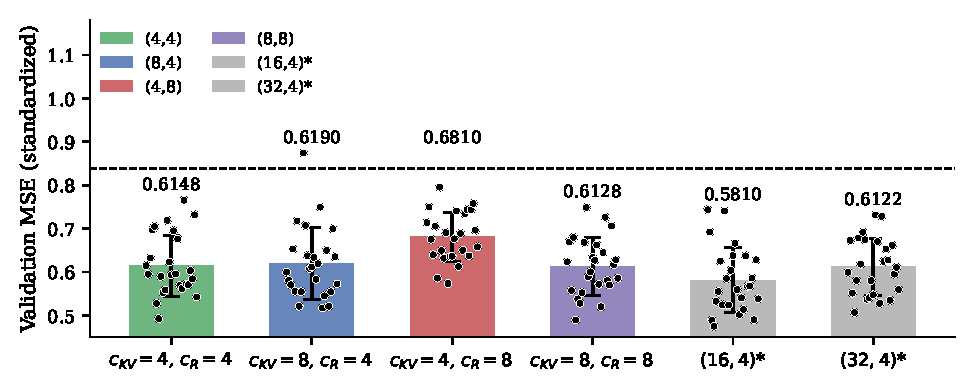
\includegraphics[width=0.92\linewidth]{figures/fig1_factorial_val.pdf}
\caption{Validation MSE by factorial cell (mean $\pm$ std over 5 paired
seeds; individual seed points shown). Lower is better. The champion corner
$(c_{KV}{=}8, c_R{=}4)$ combines coarse KV compression with fine routing.}
\label{fig:factorial}
\end{figure}

\textbf{Main effects.} Averaging over the opposite axis (Figure
\ref{fig:main-effects}): coarsening KV compression from $4{:}1$ to $8{:}1$
\emph{lowers} validation MSE by $-0.0427$ (mildly beneficial), while
coarsening routing resolution from $4{:}1$ to $8{:}1$ \emph{raises} it by
$+0.0463$ (deterioration). Both signs are consistent in 7 of 10
seed-column comparisons each.

\textbf{Pre-registered hypothesis H1} asked whether coarsening the router
deteriorates performance \emph{more} than coarsening KV compression. The
strict form is \emph{not} confirmed: the two effects are nearly equal in
magnitude ($0.0463$ vs.\ $0.0427$) and opposite in sign, so all observed
deterioration is attributable to routing while KV compression is mildly
beneficial. Both effect sizes (${\sim}0.04$) are smaller than the mean
within-cell seed standard deviation ($0.0647$; per-cell range
$0.0393$--$0.0875$), and no formal significance test was run. We therefore
report the decoupling direction as \emph{directional evidence}, not a
conclusive result (see the statistical treatment in
Section~\ref{sec:stats}; a mixed-effects model
$\mathrm{MSE} = \beta_0 + \beta_1 \log_2 c_{KV} + \beta_2 \log_2 c_R +
\beta_3 \log_2 c_{KV}\log_2 c_R + \text{random effects}$, with the main
claim requiring $\beta_2 > \beta_1$, is deferred until more cells and seeds
exist). Per-seed trajectories show the
ordering across cells is not unanimous for every seed---another reason the
champion claim is stated as ``best on mean,'' not ``best for every seed.''

\begin{figure}[t]
\centering
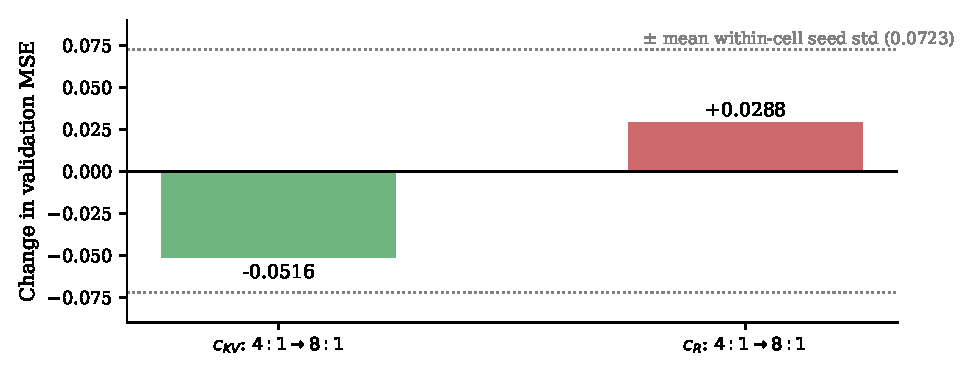
\includegraphics[width=0.92\linewidth]{figures/fig2_main_effects.pdf}
\caption{Main effects on validation MSE: $c_{KV}$ $4{:}1 \rightarrow 8{:}1$
($-0.0427$, mildly beneficial) and $c_R$ $4{:}1 \rightarrow 8{:}1$
($+0.0463$, deteriorates). Dashed lines: $\pm$ mean within-cell seed std
($0.0647$); both effects are smaller than seed noise.}
\label{fig:main-effects}
\end{figure}

\subsection{RQ2: compressed vs.\ full attention}
\label{sec:rq2}
Table~\ref{tab:baseline} compares full causal attention (Normal, 256
columns, no compression) with the two cells that anchor the family's
design corners, CSA $(4,4)$ and the champion DRRA $(8,4)$.
Every compressed cell beats Normal on mean validation
and mean test MSE, and \emph{every one of the 20 paired seed comparisons}
favors the compressed configuration (range of validation deltas
$-18.5\%$ to $-29.1\%$; the DRRA $(8,4)$ cell's advantage is the largest in 3 of
5 seeds, with CSA $(4,4)$ ahead at seeds 2024 and 99).

\begin{table}[t]
\centering
\small
\caption{Compressed vs.\ full attention (5 paired seeds, frozen protocol).
Deltas are computed on the 4-decimal means. Parameter counts are not
equalized across the three rows: Normal is a different attention class and
carries $\sim$2\% more full-model parameters.}
\label{tab:baseline}
\begin{tabular}{lccccc}
\toprule
Config & Val mean $\pm$ std & Test mean & $\Delta$val vs.\ Normal & $\Delta$test vs.\ Normal & Seeds beating Normal \\
\midrule
Normal & $0.8416 \pm 0.0799$ & 1.0814 & --- & --- & --- \\
CSA $(4,4)$ & $0.6332 \pm 0.0611$ & 0.9079 & $-24.76\%$ & $-16.04\%$ & 5 / 5 \\
DRRA $(8,4)$ & $\mathbf{0.5967} \pm 0.0710$ & $\mathbf{0.7988}$ & $-29.10\%$ & $-26.13\%$ & 5 / 5 \\
\bottomrule
\end{tabular}
\end{table}

\textbf{Wiring verification.} Because the compressed variants beating an
unmodified baseline by ${\sim}25$--$29\%$ is a surprising direction, we
audited the Normal attention implementation before reporting it: a
from-scratch naive reference (true causal masking, $1/\sqrt{d}$ scaling,
independent RoPE reimplementation) matches the module output
bit-exactly at $L{=}32$ and $L{=}64$ ($0.0$ max absolute difference) and to
$1.19 \times 10^{-7}$ at $L{=}256$ (fp32 accumulation noise); future
positions receive exactly zero weight and future-token perturbation leaves
outputs unchanged. The baseline is correctly implemented, so the comparison
stands. We also note the direction is surprising in the other sense:
compression acting as a task-appropriate inductive bias (see
Section~\ref{sec:discussion}) is a plausible but \emph{unverified}
explanation \emph{that three mechanistic probes now support descriptively}
(plan/gates/gate12/gate12\_summary.md): (i) on the delayed-copy dataset
(five channels periodic with in-window lags 96--256, plus two noise
channels), \emph{all three} models learn the exact-offset copy ---
per-channel copy MSE $0.0007$ (Normal) and $0.0013$--$0.0026$ (compressed
cells) against a noise floor of ${\approx}1.05$ --- so exact-offset recall
is not the differentiator, though Normal is ${\sim}2\times$ more precise
on the copy channels, with a mild lag gradient for the compressed cells;
(ii) on the change-point dataset, DRRA $(8,4)$ has the lowest per-window error
in \emph{every} distance-from-change bucket (the across-bucket gradient is
confounded by the generator's random-walk drift and should not be
over-read); and (iii) across the twelve datasets, the compression
advantage correlates with signal smoothness in the predicted direction
(Pearson $r = -0.29$ for DRRA $(8,4)$, $-0.35$ for CSA $(4,4)$ against lag-1
autocorrelation; $p \approx 0.3$) --- smoother series favor compression
more. These probes are descriptive ($n{=}1$ seed for (i)--(ii), $n{=}12$
for (iii)) and do not establish the mechanism.

\subsection{RQ3: cross-dataset coverage}
\label{sec:rq3}
To test whether the ETTh1 result is a single-dataset artifact, we repeated
the three-way comparison (Normal vs.\ CSA $(4,4)$ vs.\ DRRA $(8,4)$) on eleven
further datasets---three more ETT members, three large multivariate sets,
two different-dynamics sets, and three mechanistic synthetic families---under
the identical frozen protocol with the same five paired seeds (180 runs in
total; per-seed tables and the integrity audit in
plan/gates/gate3/gate3\_summary.md). Table~\ref{tab:coverage} and
Figure~\ref{fig:coverage} summarize validation MSE by dataset.

\textbf{Reading the table.} Table~\ref{tab:coverage} is transposed relative
to the earlier ones: each \emph{row} is a configuration (Normal, CSA $(4,4)$,
DRRA $(8,4)$, plus a $\Delta$val row for DRRA $(8,4)$ vs.\ Normal) and each
\emph{column} is one of the twelve datasets; a cell holds the mean
validation MSE over the five paired seeds, with the best mean per dataset
column in bold. Reading down a column compares the three models on one
dataset---e.g., ETTm2 is the suite's largest win for DRRA $(8,4)$ ($-48.4\%$),
while in the syn-delayedcopy column all three models agree within $0.001$
and Normal's mean is best. Reading across a row compares one model across
datasets, but \emph{columns are not comparable to each other}: every
dataset is standardized with its own train-only statistics, so MSE values
only have meaning within a column. The final $\Delta$val row is
scale-free (a ratio per dataset) and is therefore the row to compare across
columns; it also carries the honest exceptions---positive entries on
Exchange ($+8.6\%$) and on all three synthetic families ($+0.2\%$ to
$+3.1\%$).

The compressed configurations beat full attention on mean validation MSE in
8/12 datasets (DRRA $(8,4)$) and 7/12 (CSA $(4,4)$), but the advantage is
\emph{signal-dependent} rather than universal. The largest wins are on the
ETT family (up to $-48.4\%$ on ETTm2) and on solar-energy; both compressed
variants \emph{lose} on all three synthetic families ($+0.2\%$ to $+3.1\%$)
and on exchange-rate validation, and their test error is worse on weather
($+5.9\%$ and $+14.2\%$). This pattern is consistent with the
compression-as-inductive-bias reading: pooling adjacent timesteps is nearly
lossless on smooth, temporally redundant real-world series, while tasks
requiring exact in-window content recall (the delayed-copy probe,
known-period sinusoids) leave full attention with a slight edge. These
observations remain descriptive: five paired seeds per dataset, no
significance test, and the three rows are not parameter-equalized
($\sim$2\% full-model spread; the same stance as
Section~\ref{sec:rq2}).

\begin{table}[t]
\centering
\small
\caption{Cross-dataset validation MSE (5 paired seeds, frozen protocol;
pooled MSE in standardized units, lower is better). Models as rows,
datasets as columns; bold: best mean per dataset column. Column
abbreviations: Elec=Electricity, Traf=Traffic, Wea=Weather, Exc=Exchange,
Sol=Solar-Energy, sSin=syn-sinusoids, sCP=syn-changepts, sDC=syn-delayedcopy.
Full per-seed tables and integrity audit: plan/gates/gate3/gate3\_summary.md.}
\label{tab:coverage}
\setlength{\tabcolsep}{4pt}
\resizebox{\linewidth}{!}{%
\begin{tabular}{lrrrrrrrrrrrr}
\toprule
Model & ETTh1 & ETTh2 & ETTm1 & ETTm2 & Elec & Traf & Wea & Exc & Sol & sSin & sCP & sDC \\
\midrule
Normal    & 0.8416 & 1.9187 & 0.4285 & 1.5618 & 0.4047 & 0.5994 & 0.4460 & $\mathbf{2.9800}$ & 0.1899 & $\mathbf{0.1227}$ & $\mathbf{5.9456}$ & $\mathbf{0.2888}$ \\
CSA $(4,4)$   & 0.6332 & $\mathbf{1.3624}$ & 0.3965 & 0.9964 & $\mathbf{0.3798}$ & $\mathbf{0.5838}$ & 0.4469 & 3.1166 & $\mathbf{0.1721}$ & 0.1264 & 5.9677 & 0.2894 \\
DRRA $(8,4)$   & $\mathbf{0.5967}$ & 1.8080 & $\mathbf{0.3832}$ & $\mathbf{0.8053}$ & 0.3808 & 0.5874 & $\mathbf{0.4424}$ & 3.2350 & 0.1722 & 0.1264 & 6.0013 & 0.2894 \\
$\Delta$val DRRA $(8,4)$ vs Normal & $-29.1\%$ & $-5.8\%$ & $-10.6\%$ & $-48.4\%$ & $-5.9\%$ & $-2.0\%$ & $-0.8\%$ & $+8.6\%$ & $-9.3\%$ & $+3.1\%$ & $+0.9\%$ & $+0.2\%$ \\
\bottomrule
\end{tabular}}
\end{table}

\begin{figure}[t]
\centering
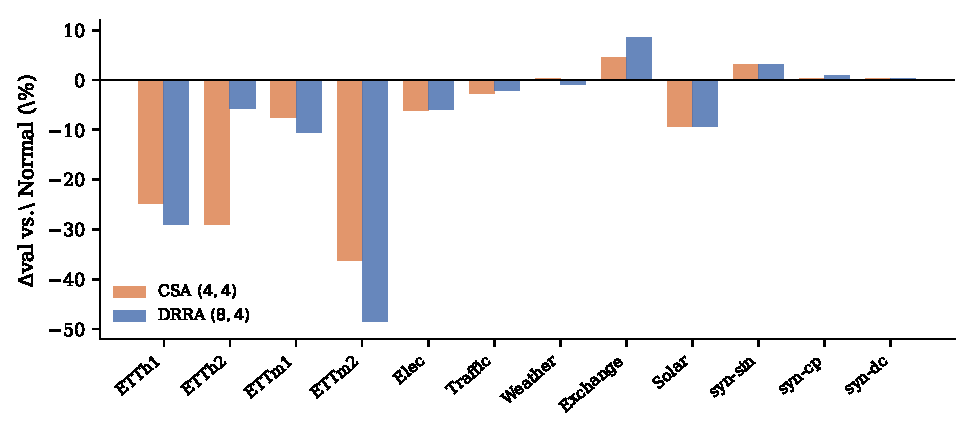
\includegraphics[width=0.92\linewidth]{figures/fig6_dataset_coverage.pdf}
\caption{Validation-MSE change vs.\ full attention by dataset (mean over 5
paired seeds): CSA $(4,4)$ (orange) and DRRA $(8,4)$ (blue). Compression helps on the
ETT family, solar, and electricity but slightly hurts on the synthetic
probes and exchange-rate validation.}
\label{fig:coverage}
\end{figure}

\subsection{Statistical treatment}
\label{sec:stats}
All comparisons above are descriptive. To make the evidentiary status
precise rather than implicit, we ran an analysis-only statistical pass on
the existing runs (no new training; log in plan/gates/gate4/gate4\_stats.md).
Per-dataset, the three comparisons (DRRA vs.\ Normal, CSA $(4,4)$ vs.\ Normal,
DRRA vs.\ CSA) were tested with exact paired Wilcoxon signed-rank tests
on validation MSE; \emph{nothing survives Holm correction across the 36
tests}, and with $n{=}5$ paired seeds the two-sided $p$-value floor is
$0.0625$, so no per-dataset effect \emph{can} reach $p < 0.05$ at this
sample size (the closest raw values are etth1 and solar at $0.0625$ in
favor of DRRA $(8,4)$; the synthetic probes are significant in the opposite
direction). Across datasets, paired sign tests on the 12 dataset means are
not significant either: DRRA $(8,4)$ beats Normal on mean validation MSE in 8/12
datasets ($p = 0.39$) and CSA $(4,4)$ in 7/12 ($p = 0.77$). The strongest
scale-free aggregate statement available is the bootstrap 95\% CI on the
mean of the per-dataset $\Delta$val vs.\ Normal: it excludes zero for both
variants (CSA $(4,4)$: $-8.9\%$ $[-16.8, -2.2]$; DRRA $(8,4)$: $-8.3\%$
$[-17.5, -0.8]$). We therefore state the results as directionally
consistent but not statistically established per dataset---the only
defensible claim at this sample size---and report these tests so that the
status is explicit rather than left to the reader. Deferred items, with
written justification in the project plan: the mixed-effects model
(Section~\ref{sec:rq1}), HAC/block-bootstrap corrections (the analysis is
at the seed level, where the five paired runs are independent, so stride-1
window overlap does not invalidate the paired tests), and TOST/ROPE (the
paper makes no equivalence claims).

\textbf{Sequence-length scaling and complexity.}
Figure~\ref{fig:lscale} sweeps the lookback $L \in \{128, \dots, 4096\}$ at
batch 1 and 32. At batch 32 the champion's advantage over Normal grows from
$-32\%$ at $L{=}512$ to $-56\%$ at $L{=}2048$ ($869$ vs.\ $1984$ ms/batch, a
$2.3\times$ speedup), and at batch 1/$L{=}4096$ it reaches $-63\%$ ($86$ vs.\
$235$ ms)---while at $L \le 256$ and batch 1 Normal is fastest (fixed overheads
again). The
empirical log-log slopes ($L \ge 512$) are $1.40$ (champion), $1.42$
(CSA $(4,4)$), and $1.72$ (Normal) at batch 32: consistent with the complexity
analysis of Section~\ref{sec:factorial}---the routing term
$O(L^2/c_R)$ keeps every cell asymptotically quadratic, with a reduced
constant for the compressed cells, and Normal approaches the quadratic
slope fastest. We therefore do \emph{not} claim subquadratic scaling. At
the extreme, batch-32/$L{=}4096$ full attention requires a ${\sim}8$ GB
score tensor and was skipped on the 16 GB machine---the practical memory
wall of dense attention that compressed attention avoids. All models
process the frozen task in under $2$ ms per sequence at batch 32 (mean
$1.6$--$1.8$ ms/seq at $L{=}256$; the $L{\ge}512$ region of the scaling
panel is where attention, not fixed overhead, dominates per-batch time).

\textbf{Compute and memory accounting.} Analytic forward MACs per sequence
(L=256, dominant terms; formulas in plan/gates/gate5/gate5\_bench.py):
Normal $76.9$M, CSA $(4,4)$ $61.7$M, DRRA $(8,4)$ $59.6$M --- the champion needs
$22\%$ fewer MACs than Normal. Two honest caveats: the wrapper MLP
($33.9$M) is the largest single block for \emph{every} model, so attention
is not the dominant compute at this scale; and measured latency differences
($-6\%$) are smaller than the MAC difference ($-22\%$) because dense-masked
CPU GEMMs are efficient relative to the extra compressor/indexer work.
Peak resident memory during a batch-32 forward burst grows by
${\sim}0.3$ GB (process watermark; parameter memory is only ${\sim}1.4$ MB
per model), and at batch-32/$L{=}4096$ the full-attention score tensor
(${\sim}8$ GB) exceeds the 16 GB machine. Training time over the fixed
10-epoch ETTh1 budget (parsed from the sweep log; medians of 5 runs):
Normal $474$ s, CSA $(4,4)$ $511$ s, DRRA $(8,4)$ $459$ s --- one DRRA run
($1417$ s) overlapped a machine-sleep window and is excluded from the
median. All latency/compute measurements are single-machine (Apple M2,
fp32, 8 threads); cross-hardware transfer (Linux x86, GPU) and model
depth/width sweeps remain future work (Appendix roadmap item~4).

\begin{figure}[t]
\centering
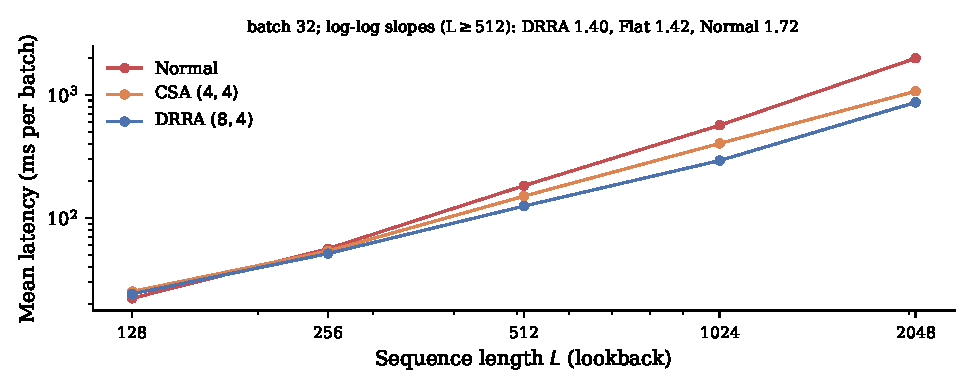
\includegraphics[width=0.92\linewidth]{figures/fig8_lscale.pdf}
\caption{Forward-pass latency vs.\ lookback length $L$ (log-log; batch 32;
mean over per-round medians). All cells are asymptotically quadratic
(routing term $O(L^2/c_R)$); the compressed cells have smaller constants
and lower empirical slopes ($1.40$/$1.42$ vs.\ $1.72$ for Normal at batch
32), and batch-32/$L{=}4096$ full attention exceeds practical memory (see
text). Measurement log: plan/gates/gate5/gate5\_bench.py +
gate5\_results.json.}
\label{fig:lscale}
\end{figure}

\subsection{Efficiency}
\label{sec:efficiency}
Table~\ref{tab:configs} gives the structural efficiency story: the
champion attends to 48 columns per query (5.3$\times$ fewer than Normal)
at 95{,}652 attention parameters---\emph{fewer} than Normal's 102{,}496---and
a full-model count 2.0\% below Normal's. Routing cost is identical for the
two $c_R{=}4$ cells regardless of $c_{KV}$, which is the deliberate
trade-off: pay the full fine-routing cost, halve the attention cost.

Table~\ref{tab:speed} reports wall-clock forward-pass latency measured
\emph{now} under the frozen protocol on the development machine, using the
alternating head-to-head protocol (all three models timed in rotation within
each round, so each round shares the same thermal/contention window; 25
rounds of 30 passes after warm-up; mean over per-round medians with 95\%
percentile bootstrap CIs, plus p90/p99 tails). The champion has the lowest
mean latency ($49.3$ ms vs.\ $52.5$ ms for Normal, $-6.1\%$; CSA $(4,4)$
$-0.7\%$), and the ordering $(8,4) < (4,4) <$ Normal replicated across a
second run, but the 95\% CIs overlap and the level shifts by
${\sim}6$--$9\%$ between runs (thermal and contention effects), so we report
the latency comparison as \emph{directional} only. Notably, the structural
5.3$\times$ column reduction does not translate into proportional wall-clock
gains at this scale: dense-masked CPU GEMMs are efficient and the
compressor/indexer add overhead. These are single-machine CPU measurements
(fp32, 8 threads); cross-hardware transfer (Linux x86, GPU) remains
follow-up work (Appendix roadmap item~4).
The pilot-era speed figures from earlier stages of this project remain
superseded and are not used here.

\textbf{Batch-size scaling.} Figure~\ref{fig:latency-scale} shows how the
comparison changes with the number of input windows processed per forward
pass (mean ms per sequence). At batch size 1 the fixed per-model overheads
(compressor, indexer) dominate and Normal is fastest ($2.5$ vs.\ $3.3$
ms/seq for DRRA $(8,4)$, $+30.8\%$). From batch 8 onward the compressed cells run
at or below Normal, and at large batches the attention-column reduction
takes over: the DRRA $(8,4)$ mean advantage over Normal is $-6.1\%$ at batch 64,
$-5.1\%$ at 100, $-10.5\%$ at 128, and $-21.1\%$ at 256 ($3.49$ vs.\ $4.42$
ms/seq). At the mid-range batches 16--32 the two are within run-to-run
noise (the scaling run shows $-0.1$ to $+0.2\%$ there while the canonical
Table~\ref{tab:speed} run shows $-6.1\%$ at batch 32). The overall pattern
is the expected signature of amortized overheads: the compression machinery
costs fixed work per pass, while the saved attention columns scale with the
batch.

\textbf{Synthesis: is the dual-rate design better?} Each table speaks to one
axis of ``better.'' Table~\ref{tab:configs} establishes the \emph{structural}
side: DRRA $(8,4)$ needs 48 attention columns (5.3$\times$ fewer than Normal),
slightly fewer parameters than Normal, and the same fine-routing candidate
count as the equal-rate cells. Tables~\ref{tab:factorial}--\ref{tab:coverage}
establish the \emph{accuracy} side: the champion beats Normal on mean
validation MSE in 8/12 datasets and has the best factorial cell on ETTh1,
with effects that are directional and, on the synthetic probes and some
datasets, reversed. Table~\ref{tab:speed} and Figure~\ref{fig:latency-scale}
establish the \emph{measured-latency} side: the champion has the lowest mean
latency at batch sizes $\ge 64$ (to $-21\%$ at 256) but is not statistically
separated from Normal at batch 32, and is slower at batch 1. Read together,
the evidence favors DRRA $(8,4)$ on every axis---geometry, parameters, accuracy
on most datasets, large-batch latency---but none of the advantages clears a
significance or noise threshold on its own, and the accuracy advantage is
dataset-dependent. We therefore state the conclusion as \emph{directional
superiority under this protocol on most datasets}, not a universal or
statistically established claim.

\textbf{Combined performance--speed view.}
Figure~\ref{fig:perf-speed} shows performance and speed \emph{together},
without collapsing them into a single score: the y-axis is the mean test
\emph{loss on ETTh1} (the frozen-task benchmark dataset, where all three
models share the same standardized scale; per-dataset losses across the
suite are \emph{not} averaged, because each dataset is standardized with
its own train-only statistics), and the x-axis is the mean forward-pass
\emph{latency} (lower latency = faster, i.e.\ the left side), at the frozen
batch 32 (left) and at batch 256 (right). Both axes are zoomed to the
measured range so the differences are visible; points are the five-seed
means, with no error bars shown. The best model in this view is the one in
the lower-left: \textbf{DRRA $(8,4)$} has the lowest mean test loss on ETTh1
($0.799$ vs.\ $0.908$ for CSA $(4,4)$ and $1.081$ for Normal) and the lowest
latency at both operating points ($49.3$ vs.\ $52.1$/$52.5$ ms at batch 32;
$892$ vs.\ $1171$/$1132$ ms at batch 256). CSA $(4,4)$ sits between the two on
both axes; Normal is upper-right (worst on both axes). Two honest readings:
at the frozen batch 32 the latency gap is a few milliseconds (within noise
at this scale), while at batch 256 DRRA $(8,4)$ is ${\sim}21\%$ faster; both
panels remain descriptive (five seeds per dataset, no significance tests,
single machine).

\begin{figure}[t]
\centering
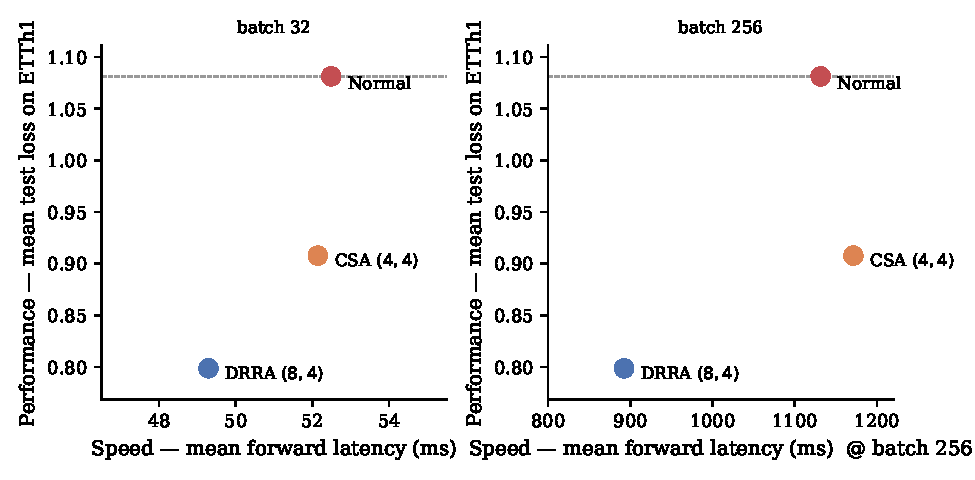
\includegraphics[width=0.92\linewidth]{figures/fig9_perf_speed.pdf}
\caption{Performance vs.\ speed: y-axis = mean test loss on ETTh1 (mean
over the five paired seeds; lower is better); x-axis = mean forward
latency (lower is faster, i.e.\ the left side); left: batch 32, right:
batch 256. DRRA $(8,4)$ is lower-left at both operating points --- the best
combined performance--speed choice --- with the separation growing at
batch 256. Measurement logs: plan/gates/gate3/gate3\_latency*.json +
gate3\_results/*.jsonl.}
\label{fig:perf-speed}
\end{figure}

\begin{figure}[t]
\centering
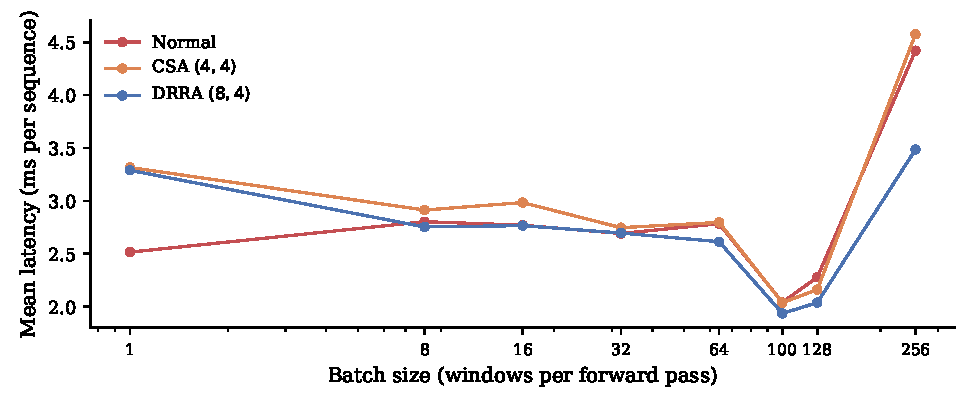
\includegraphics[width=0.92\linewidth]{figures/fig7_latency_scale.pdf}
\caption{Mean forward-pass latency per sequence vs.\ batch size under the
frozen protocol (development machine, fp32, 8 threads; mean over per-round
medians, 15 rounds $\times$ 15 passes per model per batch size). At batch
size 1 the fixed overheads of the compressor/indexer dominate and Normal is
fastest; from batch 64 onward DRRA $(8,4)$ is clearly fastest, with the gap
widening to $-21\%$ at batch 256. Measurement log:
plan/gates/gate3/gate3\_latency\_scale.py + gate3\_latency\_scale.json.}
\label{fig:latency-scale}
\end{figure}

\begin{table}[t]
\centering
\small
\caption{Forward-pass latency under the frozen protocol on the development
machine (Apple M2, 8 cores, 16 GB; CPU PyTorch 2.6.0, fp32, 8 threads).
Latency is the wall-clock time of \emph{one forward pass over a batch of 32
input windows} ($L{=}256$, $H{=}96$, $F{=}7$); per-sequence latency at this
batch size is mean$/32$ (${\approx}1.5$ ms/seq for DRRA $(8,4)$). Alternating
head-to-head protocol (25 rounds $\times$ 30 passes, warm-up excluded);
mean over per-round medians (95\% percentile bootstrap CI in brackets), with
p90/p99 tails; throughput from the mean pass time. Measurement log:
plan/gates/gate3/gate3\_latency.py + gate3\_latency.json.}
\label{tab:speed}
\begin{tabular}{lccccc}
\toprule
Model & Mean (ms) & p90 (ms) & p99 (ms) & $\Delta$mean vs.\ Normal & Throughput (batches/s) \\
\midrule
Normal & 52.5 $[50.4, 54.7]$ & 59.4 & 65.0 & --- & 19.1 \\
CSA $(4,4)$ & 52.1 $[49.2, 55.4]$ & 63.5 & 71.5 & $-0.7\%$ & 19.2 \\
DRRA $(8,4)$ & 49.3 $[47.2, 51.7]$ & 56.5 & 65.9 & $-6.1\%$ & 20.3 \\
\bottomrule
\end{tabular}
\end{table}
